\documentclass[a4paper,12pt]{article}
\usepackage[top = 2.5cm, bottom = 2.5cm, left = 2.5cm, right = 2.5cm]{geometry}
\usepackage[T1]{fontenc}
\usepackage[utf8]{inputenc}
\usepackage{multirow} 
\usepackage{booktabs} 
\usepackage{graphicx}
\usepackage[spanish]{babel}
\usepackage{setspace}
\setlength{\parindent}{0in}
\usepackage{float}
\usepackage{fancyhdr}
\usepackage{amsmath}
\usepackage{amssymb}
\usepackage{amsthm}
\usepackage{natbib}
\usepackage{graphicx}
\usepackage{subcaption}
\usepackage{booktabs}
\usepackage{etoolbox}
\usepackage{apalike}
\usepackage{minibox}
\usepackage{hyperref}
\usepackage{xcolor}
\usepackage{tcolorbox}
\usepackage{tikz}
\usepackage{pdfpages}
\usetikzlibrary{patterns}
\newcommand{\linea}{\noindent\rule{\textwidth}{1pt}}
\AtBeginEnvironment{align}{\setcounter{equation}{0}}
\newenvironment{solution}
  {\renewcommand\qedsymbol{$\square$}\begin{proof}[\textcolor{blue}{Solución}]}
  {\end{proof}}

\pagestyle{fancy}

\fancyhf{}

\lhead{\footnotesize Ecuaciones Diferenciales 2}
\rhead{\footnotesize  Rudik Roberto Rompich}
\cfoot{\footnotesize \thepage}

\begin{document}
    \thispagestyle{empty} 
    \begin{tabular}{p{15.5cm}}
    \begin{tabbing}
    \textbf{Universidad del Valle de Guatemala} \\
    Departamento de Matemática\\
    Licenciatura en Matemática Aplicada\\\\
   \textbf{Estudiante:} Rudik Roberto Rompich\\
   \textbf{E-mail:} \textcolor{blue}{ \href{mailto:rom19857@uvg.edu.gt}{rom19857@uvg.edu.gt}}\\
   \textbf{Carné:} 19857
    \end{tabbing}
    \begin{center}
        MM2030 - Ecuaciones Diferenciales 2 - Catedrático: Dorval Carías\\
        \today
    \end{center}\\
    \hline
    \\
    \end{tabular} 
    \vspace*{0.3cm} 
    \begin{center} 
    {\Large \bf Tarea 3
} 
        \vspace{2mm}
    \end{center}
    \vspace{0.4cm}
    %---------------------------
%\begin{tcolorbox}[colback=gray!15,colframe=black!1!black,title=A nice heading]
%\end{tcolorbox}

%\fbox{lol}
%---------------------------


\section{Problema 1}
Una placa rectangular de metal con lados de longitudes $a$ y $b$ y con lados (\textbf{caras}) aislados (i.e., no hay flujo de calor) se calienta a una temperatura uniforme de $u_{0}{ }^{\circ} \mathrm{C}$, manteniéndose
tres de sus lados a $0^{\circ} \mathrm{C}$ y el otro aislado. Resuelva para $u(x, y, t)$ sujeta a la condición inicial $u(x, y, 0)=100$.
\begin{solution}
Se comenzará entendiendo el problema por medio de las siguientes dos figuras:
\usetikzlibrary{patterns}
\begin{figure}[ht]
    \centering
   


% Pattern Info
 
\tikzset{
pattern size/.store in=\mcSize, 
pattern size = 5pt,
pattern thickness/.store in=\mcThickness, 
pattern thickness = 0.3pt,
pattern radius/.store in=\mcRadius, 
pattern radius = 1pt}
\makeatletter
\pgfutil@ifundefined{pgf@pattern@name@_v5u0tibg}{
\pgfdeclarepatternformonly[\mcThickness,\mcSize]{_v5u0tibg}
{\pgfqpoint{0pt}{0pt}}
{\pgfpoint{\mcSize+\mcThickness}{\mcSize+\mcThickness}}
{\pgfpoint{\mcSize}{\mcSize}}
{
\pgfsetcolor{\tikz@pattern@color}
\pgfsetlinewidth{\mcThickness}
\pgfpathmoveto{\pgfqpoint{0pt}{0pt}}
\pgfpathlineto{\pgfpoint{\mcSize+\mcThickness}{\mcSize+\mcThickness}}
\pgfusepath{stroke}
}}
\makeatother
\tikzset{every picture/.style={line width=0.75pt}} %set default line width to 0.75pt        

\begin{tikzpicture}[x=0.75pt,y=0.75pt,yscale=-1,xscale=1]
%uncomment if require: \path (0,300); %set diagram left start at 0, and has height of 300

%Shape: Cube [id:dp5983494268286695] 
\draw  [fill={rgb, 255:red, 0; green, 0; blue, 0 }  ,fill opacity=0.39 ][dash pattern={on 4.5pt off 4.5pt}] (420.4,60.04) -- (308.23,172.37) -- (180.47,172.46) -- (180.46,152.05) -- (292.63,39.72) -- (420.38,39.63) -- cycle ; \draw  [dash pattern={on 4.5pt off 4.5pt}] (180.47,172.46) -- (292.65,60.13) -- (420.4,60.04) ; \draw  [dash pattern={on 4.5pt off 4.5pt}] (292.65,60.13) -- (292.63,39.72) ;
%Straight Lines [id:da8348539716971336] 
\draw    (195.43,91.71) -- (269.51,113.16) ;
\draw [shift={(271.43,113.71)}, rotate = 196.14] [color={rgb, 255:red, 0; green, 0; blue, 0 }  ][line width=0.75]    (10.93,-3.29) .. controls (6.95,-1.4) and (3.31,-0.3) .. (0,0) .. controls (3.31,0.3) and (6.95,1.4) .. (10.93,3.29)   ;
%Straight Lines [id:da814133806997101] 
\draw    (203.78,208.88) -- (226.29,176.36) ;
\draw [shift={(227.43,174.71)}, rotate = 484.69] [color={rgb, 255:red, 0; green, 0; blue, 0 }  ][line width=0.75]    (10.93,-3.29) .. controls (6.95,-1.4) and (3.31,-0.3) .. (0,0) .. controls (3.31,0.3) and (6.95,1.4) .. (10.93,3.29)   ;
%Shape: Cube [id:dp7512885899814816] 
\draw  [fill={rgb, 255:red, 155; green, 155; blue, 155 }  ,fill opacity=0.1 ][dash pattern={on 4.5pt off 4.5pt}] (180.47,151.96) -- (292.72,39.71) -- (420.47,39.71) -- (420.47,60.12) -- (308.23,172.37) -- (180.47,172.37) -- cycle ; \draw  [dash pattern={on 4.5pt off 4.5pt}] (420.47,39.71) -- (308.23,151.96) -- (180.47,151.96) ; \draw  [dash pattern={on 4.5pt off 4.5pt}] (308.23,151.96) -- (308.23,172.37) ;
%Curve Lines [id:da2881177340231348] 
\draw [color={rgb, 255:red, 0; green, 0; blue, 0 }  ,draw opacity=0.54 ]   (403.43,133.71) .. controls (359.87,151.53) and (315.33,157.59) .. (310.56,113.08) ;
\draw [shift={(310.43,111.71)}, rotate = 445.03] [color={rgb, 255:red, 0; green, 0; blue, 0 }  ,draw opacity=0.54 ][line width=0.75]    (10.93,-3.29) .. controls (6.95,-1.4) and (3.31,-0.3) .. (0,0) .. controls (3.31,0.3) and (6.95,1.4) .. (10.93,3.29)   ;
%Shape: Rectangle [id:dp15714361951792954] 
\draw  [color={rgb, 255:red, 0; green, 0; blue, 0 }  ,draw opacity=1 ][pattern=_v5u0tibg,pattern size=7.199999999999999pt,pattern thickness=3.75pt,pattern radius=0pt, pattern color={rgb, 255:red, 253; green, 253; blue, 253}] (180.47,151.96) -- (308.23,151.96) -- (308.23,172.37) -- (180.47,172.37) -- cycle ;

% Text Node
\draw (139,60.79) node [anchor=north west][inner sep=0.75pt]  [font=\footnotesize] [align=left] {\begin{minipage}[lt]{56.822500000000005pt}\setlength\topsep{0pt}
\begin{center}
{\scriptsize Lado (cara) superior }\\{\scriptsize aislado}
\end{center}

\end{minipage}};
% Text Node
\draw (395,113.79) node [anchor=north west][inner sep=0.75pt]  [font=\footnotesize] [align=left] {\begin{minipage}[lt]{53.58643005371094pt}\setlength\topsep{0pt}
\begin{center}
{\scriptsize Lado (cara) inferior }\\{\scriptsize aislado}
\end{center}

\end{minipage}};
% Text Node
\draw (173,214.79) node [anchor=north west][inner sep=0.75pt]  [font=\footnotesize] [align=left] {\begin{minipage}[lt]{53.27071502685547pt}\setlength\topsep{0pt}
\begin{center}
{\scriptsize Lado lateral aislado}
\end{center}

\end{minipage}};
% Text Node
\draw (317,201.79) node [anchor=north west][inner sep=0.75pt]  [font=\footnotesize] [align=left] {\textcolor[rgb]{1,0,0}{*}{\tiny Los tamaños de los lados laterales han sido }\\{\tiny exagerados por motivos ilustrativos.} };
% Text Node
\draw (428.43,43.5) node [anchor=north west][inner sep=0.75pt]   [align=left] {\textcolor[rgb]{1,0,0}{*}};


\end{tikzpicture}
   \caption{Placa rectangular metálica}
\end{figure}
\begin{figure}[ht]
    \centering
    


% Pattern Info
 
\tikzset{
pattern size/.store in=\mcSize, 
pattern size = 5pt,
pattern thickness/.store in=\mcThickness, 
pattern thickness = 0.3pt,
pattern radius/.store in=\mcRadius, 
pattern radius = 1pt}
\makeatletter
\pgfutil@ifundefined{pgf@pattern@name@_ezrf09vmr}{
\pgfdeclarepatternformonly[\mcThickness,\mcSize]{_ezrf09vmr}
{\pgfqpoint{0pt}{0pt}}
{\pgfpoint{\mcSize+\mcThickness}{\mcSize+\mcThickness}}
{\pgfpoint{\mcSize}{\mcSize}}
{
\pgfsetcolor{\tikz@pattern@color}
\pgfsetlinewidth{\mcThickness}
\pgfpathmoveto{\pgfqpoint{0pt}{0pt}}
\pgfpathlineto{\pgfpoint{\mcSize+\mcThickness}{\mcSize+\mcThickness}}
\pgfusepath{stroke}
}}
\makeatother
\tikzset{every picture/.style={line width=0.75pt}} %set default line width to 0.75pt        

\begin{tikzpicture}[x=0.75pt,y=0.75pt,yscale=-1,xscale=1]
%uncomment if require: \path (0,300); %set diagram left start at 0, and has height of 300

%Shape: Axis 2D [id:dp8836634611392435] 
\draw [color={rgb, 255:red, 0; green, 0; blue, 0 }  ,draw opacity=1 ][line width=1.5]  (68.13,229.81) -- (365.13,229.81)(97.83,23.71) -- (97.83,252.71) (358.13,224.81) -- (365.13,229.81) -- (358.13,234.81) (92.83,30.71) -- (97.83,23.71) -- (102.83,30.71)  ;
%Shape: Rectangle [id:dp6128441923797413] 
\draw  [color={rgb, 255:red, 0; green, 0; blue, 0 }  ,draw opacity=1 ][fill={rgb, 255:red, 155; green, 155; blue, 155 }  ,fill opacity=0.4 ][dash pattern={on 4.5pt off 4.5pt}] (97.83,109.71) -- (267.43,109.71) -- (267.43,229.81) -- (97.83,229.81) -- cycle ;
%Shape: Rectangle [id:dp0645349541513307] 
\draw  [color={rgb, 255:red, 0; green, 0; blue, 0 }  ,draw opacity=1 ][pattern=_ezrf09vmr,pattern size=6pt,pattern thickness=3pt,pattern radius=0pt, pattern color={rgb, 255:red, 155; green, 155; blue, 155}][dash pattern={on 4.5pt off 4.5pt}] (97.83,89.71) -- (267.43,89.71) -- (267.43,109.71) -- (97.83,109.71) -- cycle ;

% Text Node
\draw (56.41,118.69) node [anchor=north west][inner sep=0.75pt]  [color={rgb, 255:red, 255; green, 255; blue, 255 }  ,opacity=1 ] [align=left] {11};
% Text Node
\draw (358,232.21) node [anchor=north west][inner sep=0.75pt]    {$x$};
% Text Node
\draw (77,21.21) node [anchor=north west][inner sep=0.75pt]    {$y$};
% Text Node
\draw (80.19,212) node [anchor=north west][inner sep=0.75pt]  [font=\scriptsize,rotate=-270.03]  {$u( 0,y,t) =0\ ^{\circ } C$};
% Text Node
\draw (144,235.21) node [anchor=north west][inner sep=0.75pt]  [font=\scriptsize]  {$u( x,0,t) =0\ ^{\circ } C$};
% Text Node
\draw (263,232.21) node [anchor=north west][inner sep=0.75pt]    {$a$};
% Text Node
\draw (82,100.21) node [anchor=north west][inner sep=0.75pt]    {$b$};
% Text Node
\draw (273.19,208) node [anchor=north west][inner sep=0.75pt]  [font=\scriptsize,rotate=-270.03]  {$u( a,y,t) =0\ ^{\circ } C$};
% Text Node
\draw (155,55.21) node [anchor=north west][inner sep=0.75pt]  [font=\scriptsize]  {$\frac{\partial u}{\partial y}\Bigl|_{y=b} =0$};


\end{tikzpicture}
   \caption{Placa en dos dimensiones}
\end{figure}
En la Figura 1, se representan las caras y un lateral aislados. Por otra parte, en la Figura 2, es la representación en dos dimensiones del problema.  
Ahora bien, el plantamiento propuesto es el siguiente: 
\begin{tcolorbox}[colback=gray!15,colframe=black!1!black,title=Condiciones - Ecuación de calor en 2D]
\begin{gather*}
    \frac{\partial u}{\partial t } =  k\left(\frac{\partial u^2}{\partial x^2 }+\frac{\partial u^2}{\partial y^2 }\right)\implies u_t=k\nabla^2u, \quad 0\leq x \leq a, \quad 0\leq y \leq b
\end{gather*}
Condiciones de frontera: 
\begin{gather*}
    u(0,y,t)=0, \quad u(a,y,t)=0, \quad u( x,0,t) =0,\quad \frac{\partial u}{\partial y}\Bigl|_{y=b} =0
\end{gather*}
Condición inicial: 
\begin{gather*}
    u(x,y,0)=100
\end{gather*}
\end{tcolorbox}
%-----------------------
Se procede con el método de separación de variables: 
\begin{gather*}
    u(x,y,t)= X(x)\cdot Y(y)\cdot T(t) = X\cdot Y \cdot T
\end{gather*}
Sustituyendo en la ecuación de calor en 2D: 
\begin{align*}
    T'XY &= k\left(X''YT+Y''XT\right)\\
    T'XY &= kT\left(X''Y+Y''X\right)\\
    \frac{T'}{kT} &= \frac{X''Y+Y''X}{XY}\\
    \frac{T'}{kT} &= \frac{X''}{X}+\frac{Y''}{Y}=-\lambda\\
\end{align*}
De la igualdad anterior, surgen tres ecuaciones diferenciales. Las primeras dos surgen de: 
\begin{gather*}
    \frac{X''}{X}+\frac{Y''}{Y} = -\lambda \quad \implies \quad  \frac{X''}{X} = -\frac{Y''}{Y} -\lambda = -\mu 
\end{gather*}

\linea 

La primera ecuación es:
\begin{gather}
    \frac{X''}{X}= -\mu \quad \implies \quad \fbox{$X''+\mu X =0$}
\end{gather}
(1) Se encuentra sujeta a las condiciones: 
$$X(0)=0, \quad X(a)=0 $$

Cuando $\mu< 0$ y $\mu=0$ las soluciones se trivializan, por lo que solo se analizará el caso en el que $\mu >0$. Entonces, la solución de (1) es:
$$ X(x) = A\cos \sqrt{\mu} x + B\sin \sqrt{\mu} x $$
 Aplicando las condiciones de frontera: 
 $$X(0)= A\cos 0 + B\sin 0 = 0 \implies A=0$$
 $$X(a)= B\sin\sqrt{\mu}a$$
 Para encontrar la relación de $\sqrt{\mu}a$ se propone: 
 $$\sqrt{\mu} a= n\pi \implies \sqrt{\mu}=\frac{n\pi}{a}$$
 Por lo tanto, la solución general es: 
\begin{gather*}
    \fbox{$X_n(x)= \sin\frac{n\pi}{a}x,\qquad n=1,2,3,... $}
\end{gather*}
%---------------------
\linea 

La segunda ecuación:
\begin{gather}
    -\frac{Y''}{Y} -\lambda = -\mu\quad \implies \quad Y'' +\underbrace{(\lambda -\mu )}_{P}Y =0 \implies \fbox{$Y'' + PY=0$}
\end{gather}

(2) Se encuentra sujeta a las condiciones de frontera: 
$$Y(0)=0, \quad \frac{\partial u}{\partial y}\Big| _{y=b}=0$$

Cuando $P<0$ y $P=0$ las soluciones se trivializan, por lo que solo se analizará el caso en el que $P>0$. Entonces, la solución de (2) es: 
$$Y(y)= C\cos\sqrt{P}y+D\sin\sqrt{P}y$$
$$Y'(y)= -\sqrt{P}C\sin \sqrt{P}y+\sqrt{P}D\cos \sqrt{P}y $$
Aplicando las condiciones de frontera: 
$$Y(0)=C\cos 0+ D\sin = 0\implies C=0$$
$$Y'(b)= \sqrt{P}D\cos \sqrt{P}b$$
\textbf{Nótese} que $D$ no puede ser 0; ya que solo nos interesan las soluciones triviales. Es decir $\cos\sqrt{P}y =0$. Para encontrar la relación de $\sqrt{P}b$, se propone: 
$$\sqrt{P}b= \pi \left(m-\frac{1}{2}\right)\implies \sqrt{P}= \frac{\pi}{b}\left(m-\frac{1}{2}\right)$$
Por lo tanto, la solución general es: 
\begin{gather*}
    \fbox{$Y_m(y)= \sin\frac{\pi}{b}\left(m-\frac{1}{2}\right)y$}
\end{gather*}

\linea 

%-----------------------
Por otra parte, la tercera ecuación es: 
\begin{gather}
    \frac{T'}{kT}=-\lambda \quad \implies \quad \fbox{$T' +\lambda k T=0$}
\end{gather}
La solución de la ecuación diferencial es: 
\begin{gather}
    T(t)= Ee^{-\lambda k t}
\end{gather}
Ahora, notamos que previamente se había propuesto $P=\lambda-\mu$. Despejando para $\lambda$, se tiene $\lambda = P+\mu$. En donde $P=\left[\frac{\pi}{b}\left(m-\frac{1}{2}\right)\right]^2$ y $\mu = \left(\frac{n\pi}{a}\right)^2$. Entonces:
\begin{align*}
    \lambda &= \left[\frac{\pi}{b}\left(m-\frac{1}{2}\right)\right]^2+\left(\frac{n\pi}{a}\right)^2\\
    &= \pi^2\left[\frac{1}{b^2}\left(m-\frac{1}{2}\right)^2+\frac{n^2}{a^2}\right]
\end{align*}

Por lo tanto, sustituyendo en (4) la solución general es: 
\begin{gather}
    \fbox{$T_{mn}(t) = \exp\left(-k\pi^2\left[\frac{1}{b^2}\left(m-\frac{1}{2}\right)^2+\frac{n^2}{a^2}\right]t\right)$}
\end{gather}

\linea 

Ahora, se tiene que, para $m,n=1,2,3,...$: 
\begin{align*}
    u_{mn}(x,y,t)&= X(x)\cdot Y(y)\cdot T(t)\\
    &= \sin\left(\frac{n\pi}{a}x\right)\cdot \sin\left(\frac{\pi}{b}\left(m-\frac{1}{2}\right) y \right)\cdot \exp\left(-k\pi^2\left[\frac{1}{b^2}\left(m-\frac{1}{2}\right)^2+\frac{n^2}{a^2}\right]t\right)
\end{align*}

\linea 

Aplicando el principio de superposición: 
\begin{align*}
    u(x,y,t) &= \sum_{m=1}^\infty\sum_{n=1}^\infty A_{mn}u_{mn}(x,y,t)\\
    &= \sum_{m=1}^\infty\sum_{n=1}^\infty A_{mn} \sin\left(\frac{n\pi}{a}x\right)\cdot \sin\left(\frac{\pi}{b}\left(m-\frac{1}{2}\right) y \right)\cdot \exp\left(-k\pi^2\left[\frac{1}{b^2}\left(m-\frac{1}{2}\right)^2+\frac{n^2}{a^2}\right]t\right)
\end{align*}

\linea 

Aplicando la condición inicial en donde $t=0$, se tiene: 

\begin{align*}
    100 &= \sum_{m=1}^\infty\sum_{n=1}^\infty u_{mn}(x,y,0)\\
    &= \sum_{m=1}^\infty\sum_{n=1}^\infty A_{mn} \sin\left(\frac{n\pi}{a}x\right)\cdot \sin\left(\frac{\pi}{b}\left(m-\frac{1}{2}\right) y \right)
\end{align*}

Ahora bien, se considerará al la relación de ortogonalidad para el seno, por lo que se tiene:

\begin{align*}
A_{m n} &=\frac{4}{a b} \int_{0}^{a} \int_{0}^{b} 100 \sin \left(\frac{n \pi}{a}x\right) \sin \left(\frac{\pi}{b}\left(m-\frac{1}{2}\right) y \right) d y d x \\
&=\frac{400}{a b} \int_{0}^{a} \sin \left(\frac{n \pi}{a}x\right) d x \int_{0}^{b} \sin \left(\frac{\pi}{b}\left(m-\frac{1}{2}\right) y \right) d y \\
&=\frac{400}{a b} \frac{L}{n \pi}(\cos (n \pi)-1) \frac{2 b}{(2 m-1) \pi}\left(\cos \left(\left(m-\frac{1}{2}\right) \pi\right)-1\right) \\
&=\frac{800}{n(2 m-1) \pi^{2}}\left(1-(-1)^{n}\right) \\
\text { Entonces } A_{m 2 n}=& 0 \text { y por lo tanto: } \\
\qquad A_{m 2 n-1} &=\frac{1600}{(2 n-1)(2 m-1) \pi^{2}}
\end{align*}

Finalmente, el resultado: 
$$
\begin{array}{r}
u(x, y, t)=\sum_{m=1}^{\infty} \sum_{n=1}^{\infty} \frac{1600}{(2 n-1)(2 m-1) \pi^{2}} \sin \left(\frac{(2 n-1) \pi x}{a}\right) \sin \left(\frac{(2 m-1) \pi y}{2 b}\right) \\
\cdot \exp \left(-\left(\frac{(2 m-1)^{2}}{4 b^{2}}+\frac{(2 n-1)^{2}}{a^{2}}\right) \kappa \pi^{2} t\right)
\end{array}
$$
\end{solution}
\newpage 
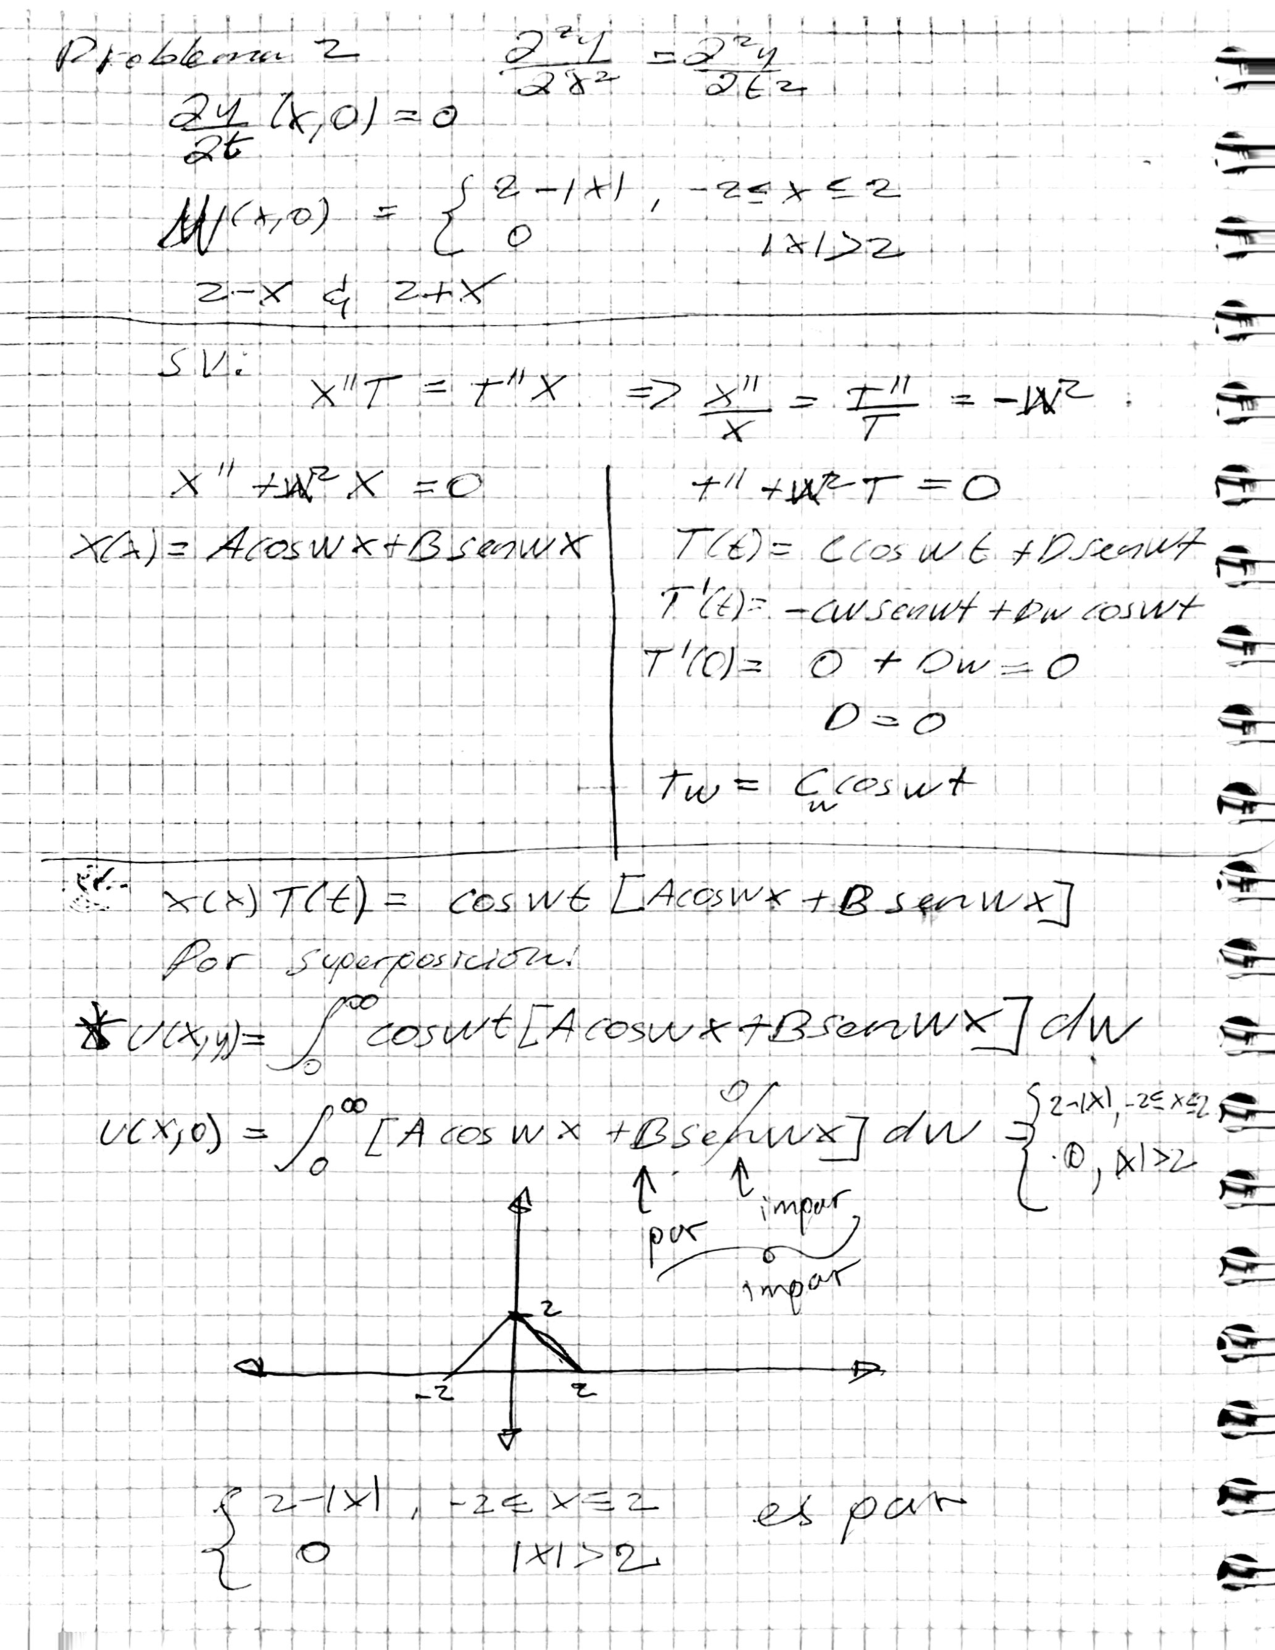
\includepdf[pages=-]{lol.pdf}

%---------------------------
%\bibliographystyle{apalike}
%\bibliography{sample.bib}

\end{document}